% !Mode:: "TeX:UTF-8"

\documentclass[11pt, a4paper]{article}
%\usepackage{xltxtra,fontspec,xunicode}
\usepackage{amsmath}
\usepackage{amssymb}
\usepackage{breqn}
\usepackage{autobreak}
\usepackage{braket,mleftright}
\usepackage{amsfonts}
\usepackage[section]{placeins}
\usepackage{float}
\usepackage{siunitx}

\usepackage{indentfirst}
\usepackage{caption}

\usepackage{geometry}
\usepackage{graphicx}

\geometry{top=1in, bottom=1in, left=1in, right=1in}
\linespread{1.5}

\DeclareMathOperator*{\argmax}{argmax}
\DeclareMathOperator*{\argmin}{argmin}

\newcommand{\degc}{$\,^\circ$C}

\begin{document}

\title{Weekly Report}
\author{Zhuoran Qiao}
\date{\today}

\maketitle
\section{One-dimensional free energy landscape}

To evaluate transiton path statistics for free energy landscapes with multi intermediate barriers,
 following toy landscapes were constructed(Figure \ref{fig:FEL}). Free energy difference between source/sink and barrier top is $5.37kT$.

\begin{figure}[h]
  \noindent\makebox[\textwidth]{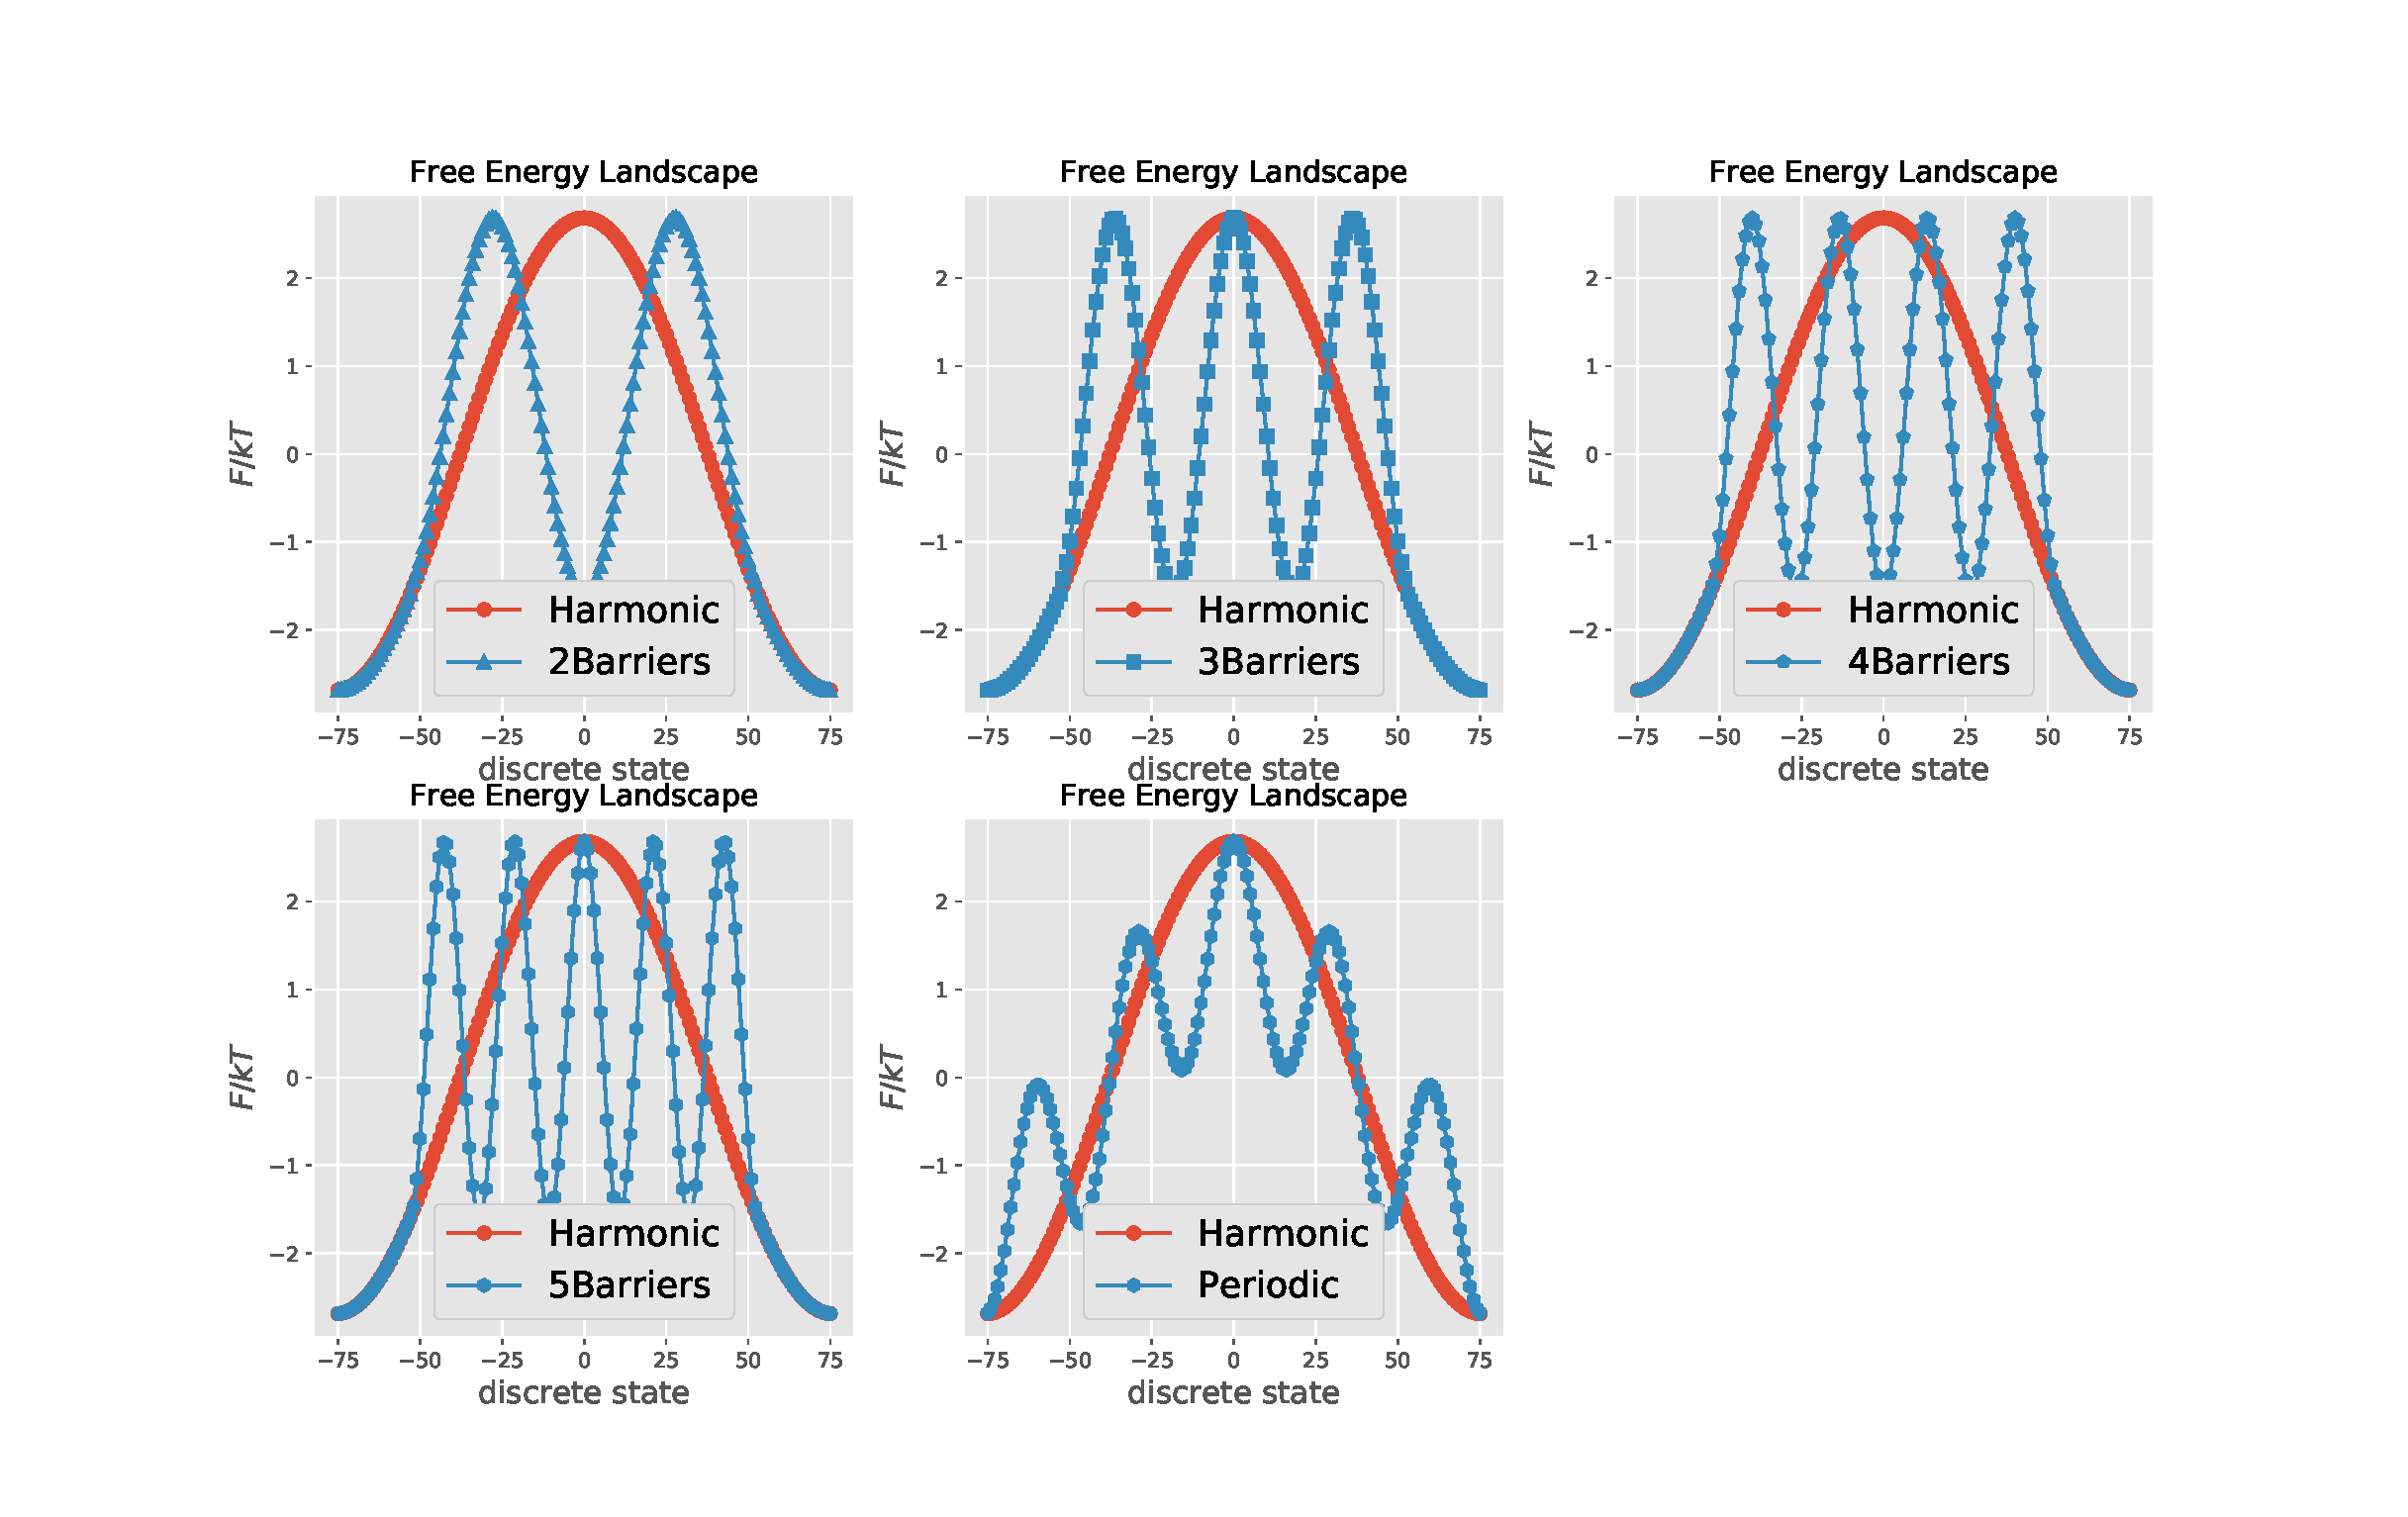
\includegraphics[width=\paperwidth]{FELs.eps}}
  \caption{Model free energy landscapes.}
  \label{fig:FEL}
\end{figure}

\section{Transition-path transit time distribution}

Ultilizing Kinetic Monte Carlo simulation for above-mentioned 1-d discrete states model, we sampled 10000
 transition-path trajectories and calculated distribution of transiton-path transit times $p(t_{AB})$ for each model landscapes.

\begin{figure}[htp]
  \noindent\makebox[\textwidth]{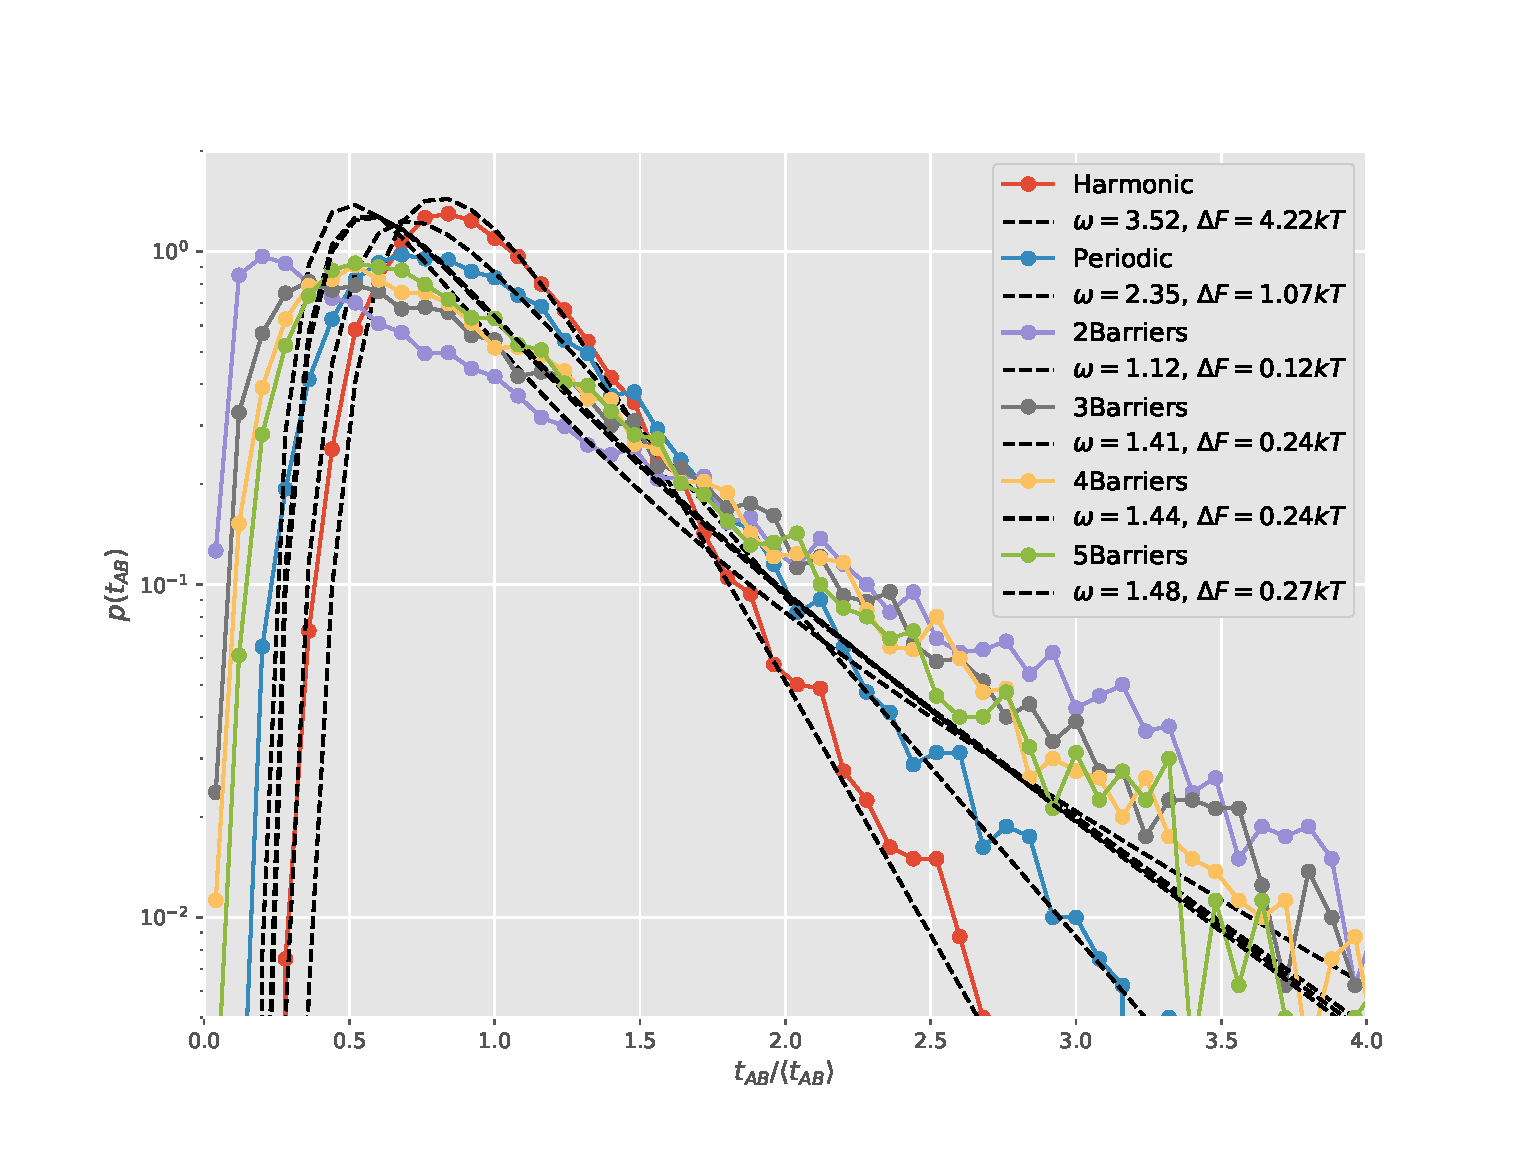
\includegraphics[width=550pt]{Transit_Time_distribution_log.eps}}
  \caption{Transition-path transit time distribution}
  \label{fig:tpt_time}
\end{figure}

For each transit time distribution, the apparent force constant of the barrier $\omega$ was determined by fitting the decay constant $\omega^{-1}$ of the asymptotic exponential tail($p(t_{AB}>1.5)$); barrier height $\Delta F$ was
 then determined by fitting theoretial expression of $p(t_{AB})$ to simulation distribution of transit times. We demonstrated that even for the harmonic landscape, deviation from theoretial expression for parabolic barrier crossing is
 non-negligible; for multi-harmonic barriers model, significant deviation from theoretical distribution was observed,resulting in much smaller and relatively unphysical fitting result for barrier height $\Delta F$.

We also calculated the probability density $P(TP|x)$ that an arbitrary trajectory crossing state $x$ is a transiton path trajectory;

\section{Finite time displacement distribution}

\begin{figure}[htp]
  \noindent\makebox[\textwidth]{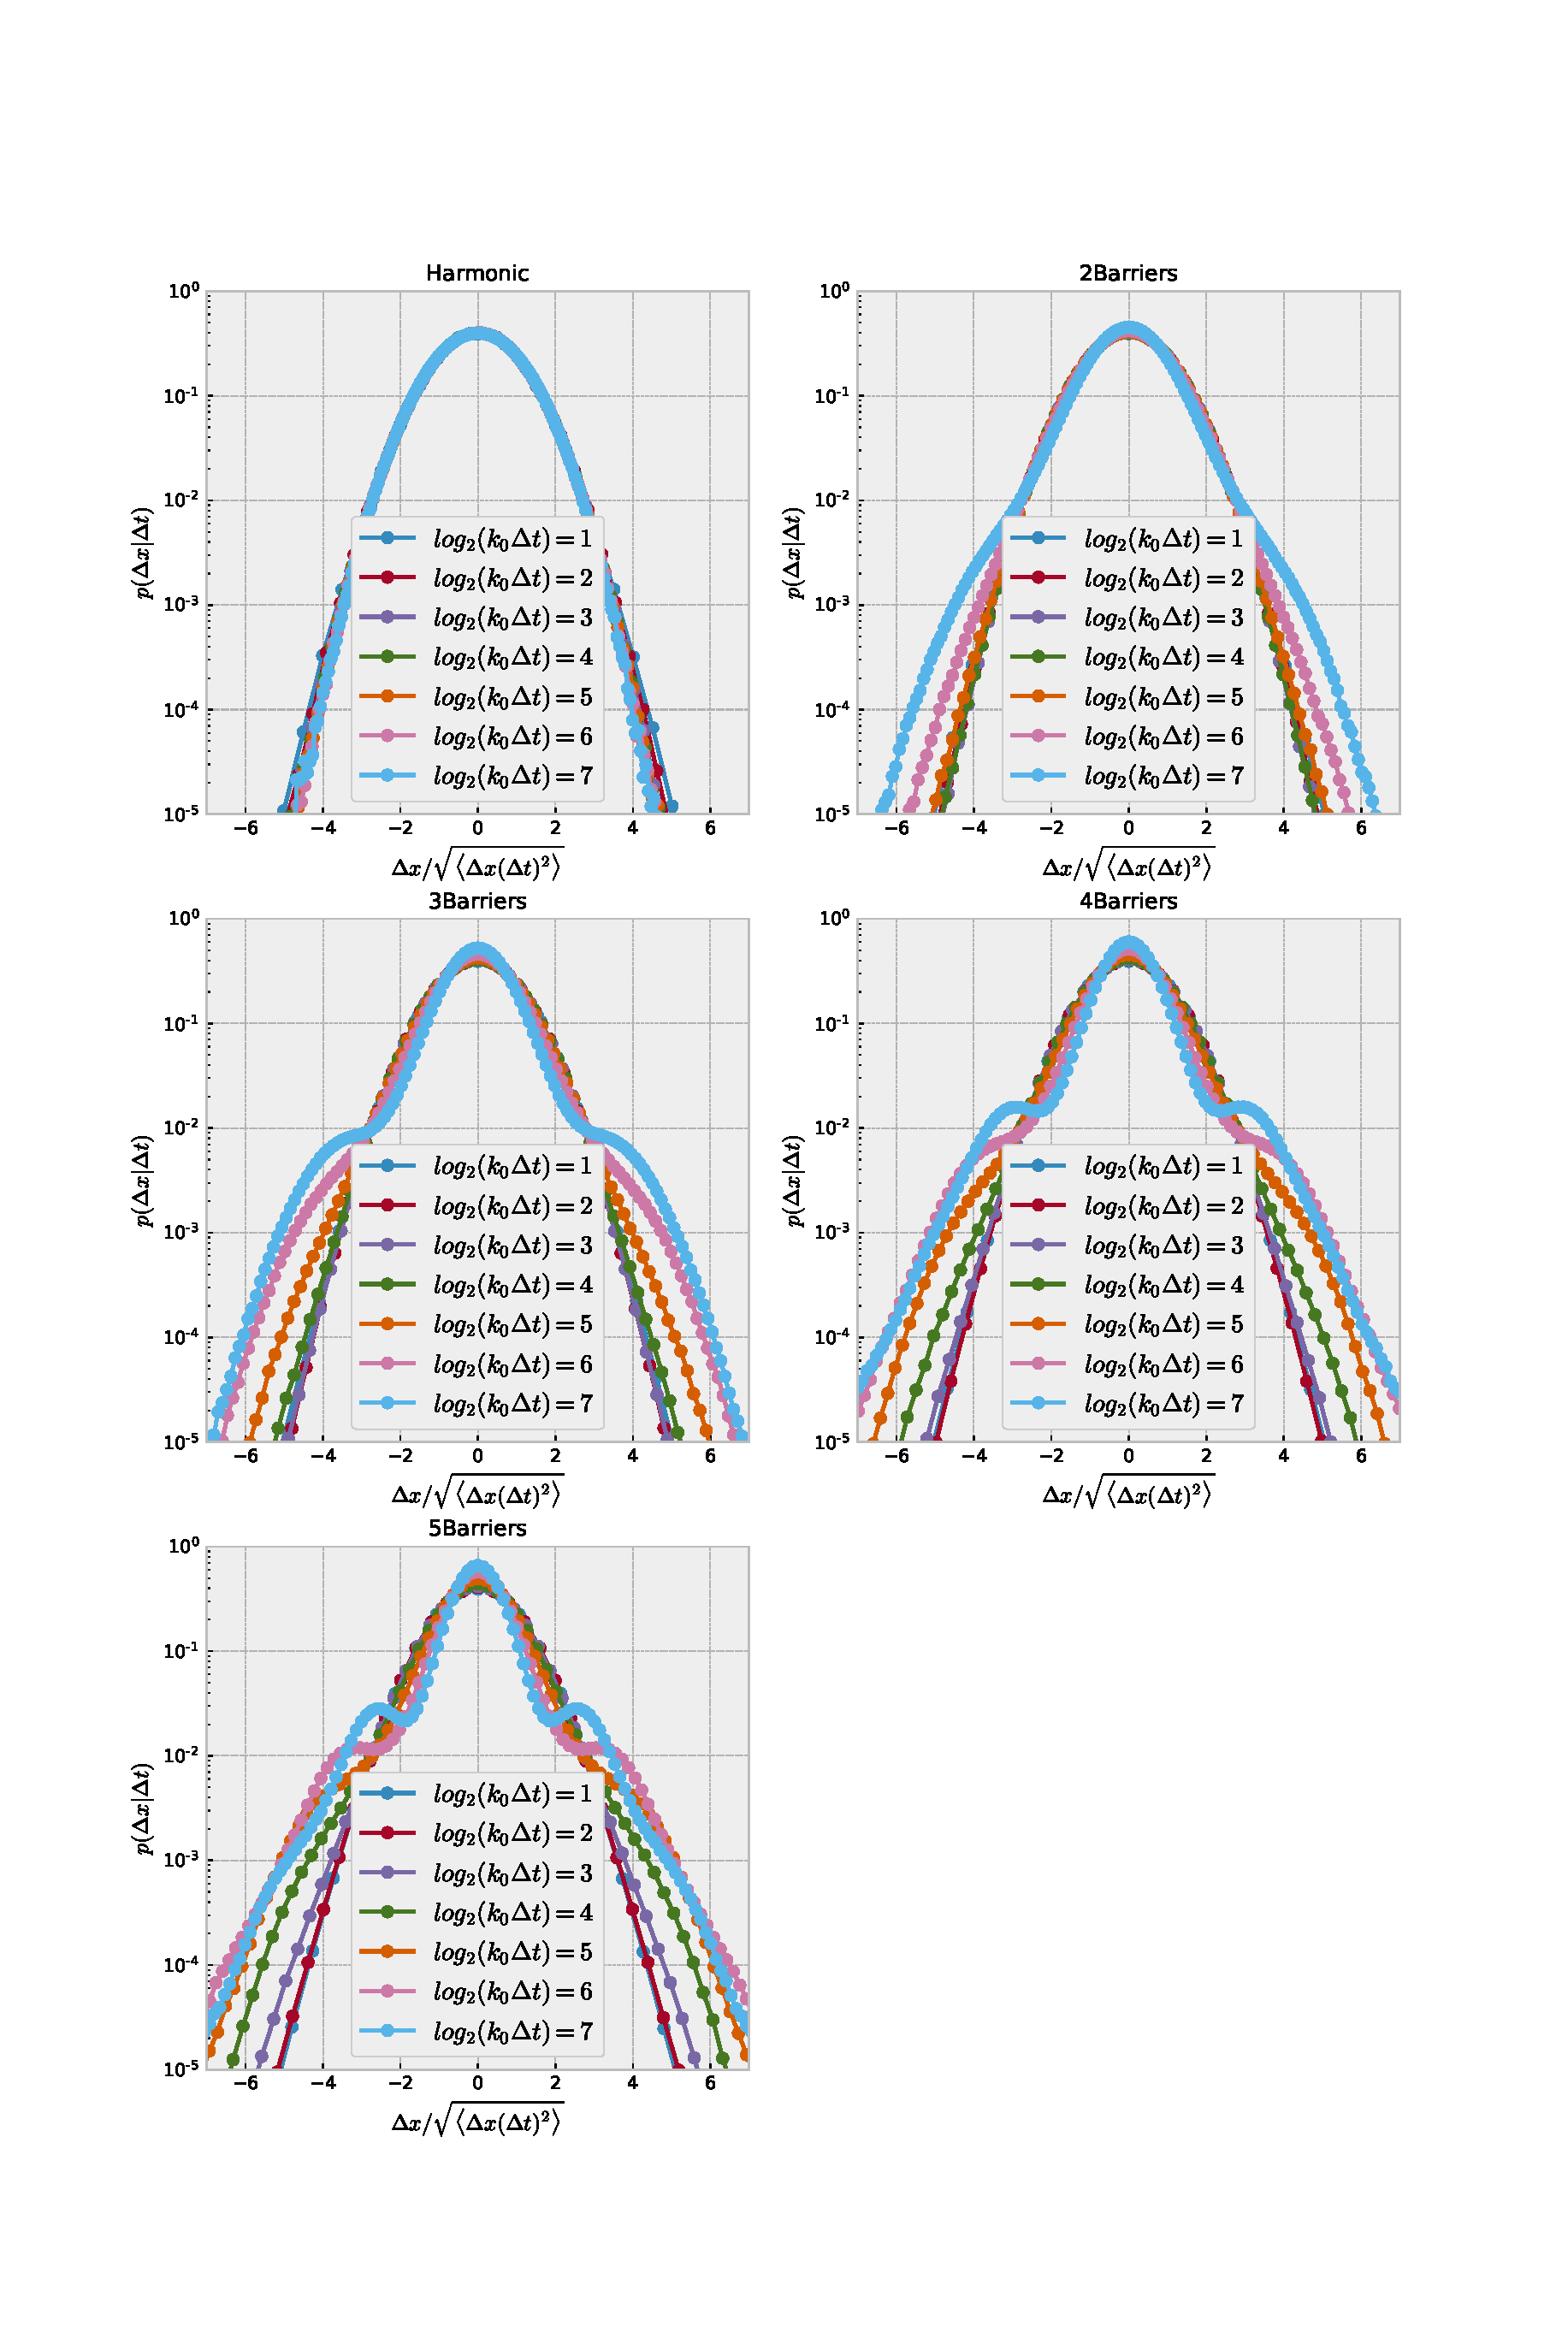
\includegraphics[width=480pt]{Finite_time_Displacement.eps}}
  \caption{Distribution of finite time displacements.}
  \label{fig:dx}
\end{figure}

In order to examine when the one-dimensional coordinate projection could be recognized as effective reaction coordinate,
we then examine the probability distribution of committors for transition path trajectories $p(q|TP)$, for which a single peak of probability $p(q|TP)$ have been ultilized as a indicator for 'good' reaction coordinates.
 Firstly, We found that for harmonic toy model, the shape of $p(q|TP)$ is very sensitive to the definition of source/sink region. For illustration, $p(q|TP)$ for two different selection
  of source/sink regions was compared: in the first case, only two free energy minimum was indentified as source or sink\textbf{(S1)}; in the second case, only the barrier top was
  defined as the transition path, while other two region of the free energy landscape was calssified as source/sink\textbf{(S2)}.

local linked


\small
\bibliographystyle{pkuplain}
\bibliography{ref}



\end{document}
